\documentclass[10pt]{article}
\usepackage{icmlko}

\icmlmeta{IP 파운데이션 월드모델}{224}{날짜는 안 바뀌지만 아직 없었다}{노트 223이 ``날짜라서 정의로 누출이 없다''고 적었다. 가드가 틀렸다고 했고 가드가 맞았다. 그리고 그 김에 판이 두 종류의 라벨을 섞고 있는 것이 드러났다}

\begin{document}

\twocolumn[
\icmlheader

\begin{abstract}
노트 223이 웹툰 초기 화 축을 만들고 \textbf{``게재일은 사후에 안 바뀌므로
정의로 누출이 없다''}고 적었다. \textbf{틀렸다.} 시점 가드가 세 축을 모두
사후로 잡았고, 재 보니 그렇다 --- \textbf{첫 스무 화는 연재 시작 후 중앙
133일(19주 · 4.4개월) 뒤에야 완성된다.} 학습 구간 안에서도 125편(4.5\%)은
스무째 화가 $T$ 이후다. \textbf{``날짜라서 안 바뀐다''와 ``그 날짜를 예측
시점에 알 수 있다''는 다른 말이고 나는 둘을 섞었다.} 이 프로젝트의 예측
시점은 출시 전이므로(팝업 오픈 전이 출발점이다) \textbf{그 축은 사후이고
채택하지 않는다} --- 노트 223의 $+$0.0294($t{=}4.5$) · $+$0.0623
($t{=}7.6$)은 \emph{다른 과제}의 수다. 갈래로 남긴다: 출시 전 예측이냐,
초기 스무 화를 본 뒤의 예측이냐. \textbf{과제를 바꾸는 결정이지 축을
고르는 결정이 아니다.} 그리고 그 김에 더 큰 것이 나왔다. 평가 점수 축을
다섯 도메인에서 재니 \textbf{라벨의 성질로 완벽하게 갈린다} --- 선호형
라벨(웹툰 즐겨찾기 $+$0.506 · 만화 popularity $+$0.386 · 세계애니
$+$0.363)과 양형 라벨(애니 리뷰 수 $-$0.038 · 모바일 평점 수 $+$0.057)
사이에 \textbf{겹침이 없다.} 첫 설명(``평점이 압축돼 있어서'')은
반증됐다 --- \textbf{웹툰이 사분위 폭 0.021 로 제일 좁은데 상관은 제일
세다.} 남는 읽기는 \textbf{평균 평점은 품질을 재고 리뷰 수 · 평점 수는
도달을 잰다}는 것이다. 그러면 판 자체가 갈린다 --- \textbf{선호형이 몫
39.4\%(가중 $\rho$ 0.4132) · 양형이 60.6\%(0.4883)} 이고 선호형이 0.075
더 어렵다. \textbf{제일 큰 도메인(웹툰 27.7\%)이 선호형이면서 $\rho$ 가
제일 낮다.} 노트 209$\sim$212가 라벨의 시계와 누적성을 다뤘지만
\textbf{라벨이 두 종류라는 것에는 이름을 붙인 적이 없다.}
\end{abstract}
]

\begin{figure*}[t]
\centering
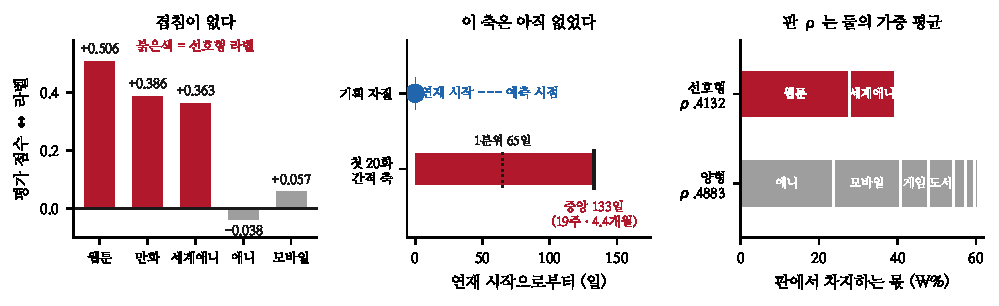
\includegraphics[width=\textwidth]{figs/twokinds.pdf}
\caption{왼쪽 --- 라벨 성질로 갈리고 겹침이 없다. 가운데 --- 그 축은
예측 시점에 아직 없었다. 오른쪽 --- 판이 두 종류의 가중 평균이다.}
\end{figure*}

\section{가드가 맞았다}

\claimx{\textbf{노트 223이 ``게재일은 사후에 안 바뀌므로 정의로 누출이
없다''고 적었는데 틀렸다.} 시점 가드가 \texttt{wt\_early\_span} ·
\texttt{cadence} · \texttt{gapvar} 셋을 모두 사후로 잡았다.}{가드는 손으로
관리하는 출처 표(\texttt{lab/provenance.py} 의 \texttt{WHEN})를 보고
\textbf{등록 안 된 축을 사후로 본다.} 기본값이 옳은 방향이다 --- 선언하지
않은 것을 사전으로 봐 주지 않는다.}

\begin{table}[t]
\centering\tsize
\caption{웹툰 2,800편. 연재 시작에서 스무째 화까지.}
\begin{tabular}{lr}
\toprule
1분위 & 65일 \\
\textbf{중앙} & \textbf{133일 (19주 · 4.4개월)} \\
3분위 & 133일 \\
\midrule
학습 구간인데 스무째 화가 $T$ 이후 & 125편 (4.5\%) \\
\bottomrule
\end{tabular}
\end{table}

\claimx{\textbf{이 축은 연재 시작 시점에 존재하지 않는다} --- 중앙
4.4개월 뒤에 완성된다. \textbf{``날짜라서 안 바뀐다''와 ``그 날짜를 예측
시점에 알 수 있다''는 다른 말이고 나는 둘을 섞었다.}}{노트 141이 시점
층을 세울 때 든 예가 ``지금 긁은 스냅샷''이었다 --- 값이 변하는 것이
문제라고 읽기 쉬운데, \textbf{진짜 기준은 \emph{그때 있었나}다.}}

\claimx{\textbf{채택하지 않는다.} 이 프로젝트의 예측 시점은 출시
전이므로(팝업 오픈 전이 출발점이다) 노트 223의 $+$0.0294 · $+$0.0623 은
\emph{다른 과제}의 수다.}{\textbf{갈래로 남긴다} --- 출시 전 예측이냐
초기 스무 화를 본 뒤의 예측이냐. \textbf{과제를 바꾸는 결정이지 축을
고르는 결정이 아니고, 점수가 큰 쪽으로 기울면 안 되는 종류다.}}

\section{판이 두 종류를 섞고 있었다}

\begin{table}[t]
\centering\tsize
\caption{평가 점수 축(덮음 99$\sim$100\%).}
\begin{tabular}{llrr}
\toprule
& 라벨 & 성질 & $\leftrightarrow$라벨 \\
\midrule
\textbf{웹툰} & \texttt{y\_favorite} & 선호 & \textbf{$+$.506} \\
\textbf{만화} & \texttt{y\_popularity} & 선호 & \textbf{$+$.386} \\
\textbf{세계애니} & \texttt{y\_popularity} & 선호 & \textbf{$+$.363} \\
\midrule
애니 & \texttt{y\_review} & 양 & $-$.038 \\
모바일 & \texttt{y\_rating\_count} & 양 & $+$.057 \\
\bottomrule
\end{tabular}
\end{table}

\claimx{\textbf{라벨의 성질로 완벽하게 갈린다} --- 선호형 셋이
$+$0.36$\sim$$+$0.51, 양형 둘이 $-$0.04$\sim$$+$0.06 이고 \textbf{겹침이
없다.}}{다섯 도메인 모두 평가 점수가 99$\sim$100\% 덮여 있다 ---
\textbf{덮음이 아니라 대상이 문제다.}}

\claimx{\textbf{첫 설명은 반증됐다.} ``평점이 압축돼 있어서''라고 봤는데
\textbf{웹툰이 사분위 폭 0.021 로 제일 좁은데 상관은 제일 세다}(애니
0.120 대 세계애니 0.139 인데 $-$0.038 대 $+$0.363).}{남는 읽기:
\textbf{평균 평점은 품질을 재고 리뷰 수 · 평점 수는 도달을 잰다.}
품질 축이 도달형 라벨을 못 맞히는 것은 결함이 아니라 \emph{다른 것을
재기} 때문이다.}

\begin{table}[t]
\centering\tsize
\caption{판을 라벨 성질로 가르면.}
\begin{tabular}{lrrl}
\toprule
& 몫 & 가중 $\rho$ & 도메인 \\
\midrule
\textbf{선호형} & \textbf{39.4\%} & \textbf{.4132} & 웹툰 · 세계애니 \\
양형 & 60.6\% & .4883 & 애니 · 모바일 · 게임 \\
& & & 도서 · 펀딩 · 팝업 · 아이돌 \\
\bottomrule
\end{tabular}
\end{table}

\claimx{\textbf{판 $\rho$ 는 두 과제의 가중 평균이고 선호형이 0.075 더
어렵다.} 그리고 \textbf{제일 큰 도메인(웹툰 27.7\%)이 선호형이면서
$\rho$ 가 제일 낮다.}}{노트 222의 천장표에서 웹툰이 1 위($+$0.1769)였던
것의 절반은 이것이다 --- \textbf{웹툰이 어려운 것이 아니라 선호를 재는
것이 어렵다.}}

\claimx{\textbf{노트 209$\sim$212가 라벨의 시계와 누적성을 다뤘지만
라벨이 두 종류라는 것에는 이름을 붙인 적이 없다.}}{그래서 ``라벨을 고정
창으로''(노트 210)가 두 종류에 같은 처방으로 적용됐다 --- \textbf{게임은
양형이라 30일 창이 맞았지만, 선호형에 창을 씌우는 것이 같은 뜻인지는 안
쟀다.}}

\section{애니는 포화한다}

\begin{table}[t]
\centering\tsize
\caption{화 간격 축을 넣으면(노트 223의 사후 갈래 안에서).}
\begin{tabular}{lrrrr}
\toprule
& F6 & F18 & 웹툰 & 애니 \\
\midrule
채택 상태 & .4250 & .4408 & .3361 & .4713 \\
웹툰만 & .4450 & \textbf{.4704} & \textbf{.4561} & .4693 \\
웹툰$+$애니 & .4356 & \textbf{.4733} & .4496 & \textbf{.4896} \\
\bottomrule
\end{tabular}
\end{table}

\claimx{\textbf{애니를 더해도 판은 $+$0.0026 뿐이다}($+$0.4704 $\to$
$+$0.4733). 애니 자신은 $+$0.4713 $\to$ $+$0.4896 으로 $+$0.018
오르는데.}{\textbf{노트 217의 포화 법칙 그대로다} --- 애니 바탕
$\rho$ 가 이미 0.47 이라 더할 것이 적다. 그리고 \textbf{F6 능형은 오히려
$-$0.0094 잃는다}(두 도메인에만 있는 열을 풀링이 못 쓴다).}

\begin{table}[t]
\centering\tsize
\caption{남은 것.}
\begin{tabular}{ll}
\toprule
\textbf{두 과제} & 선호형·양형을 갈라 판을 둘로 적을 것 \\
\textbf{출시 전 축} & 웹툰에 진짜 사전 축이 있나(작가·슬롯) \\
사후 갈래 & 초기 성과 뒤 예측을 별도 판으로 둘 것인가 \\
\bottomrule
\end{tabular}
\end{table}

첫 줄이 제일 값이 크고 값이 안 든다. \textbf{판 $\rho$ 하나로 두 과제를
평균하면 어느 쪽이 나아졌는지 모른다.} 이번 사이클만 해도 계열 질의 고침
(노트 222)이 어느 쪽을 도왔는지, 검색 덮음 채움(노트 221)이 어느 쪽을
해쳤는지 안 갈랐다. \textbf{선호형 $\rho$ 와 양형 $\rho$ 를 판 옆에 나란히
적으면 그것이 바로 보인다} --- 노트 211이 도메인별 달력 몫을 모니터에
올리자고 한 것과 같은 성질이고, 그때는 안 했다. \textbf{이번에는 판정치를
바꾸는 것이 아니라 판정치를 \emph{둘로 적는} 것이므로 순위 규칙을 안
건드린다.}

\end{document}
